
\documentclass{article}
\usepackage{polski}
% \usepackage{babel}
\usepackage{amsmath} % for maths
\usepackage{graphicx} % images
\usepackage{subcaption} % subimages
\usepackage{geometry}
\geometry{
	a4paper,
	total={150mm,267mm},
	left=30mm,
	top=15mm,
}
\setcounter{section}{4}

\title{Sprawozdanie nr 2\\Analiza Obrazów}
\date{2020-??-??}
\author{Tomasz Rajchel}
	
	
\begin{document}
	\maketitle
	\pagenumbering{gobble}

	\tableofcontents
	\newpage
	\pagenumbering{arabic}
	
	\section{Laboratorium 5 - Morfologie}
	\subsection{Wstęp}
		\begin{center}
		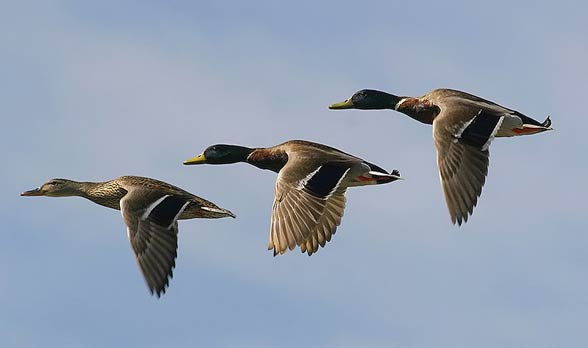
\includegraphics[width=\linewidth]{../../pictures/kaczki.jpg}
		\captionof{figure}{Obraz bazowy}
	\end{center}

	\begin{center}
		\includegraphics[width=\linewidth]{../../lab05/ducks_detection.png}
		\captionof{figure}{Wykrywanie obiektów.}
		\label{fig:cat_gray}
	\end{center}
	
	\section{Laboratorium 6 - Współczynniki geometryczne}
	\subsection{Wstęp}
	
	\section{Laboratorium 7 - Klasyfikacja obiektów przy użyciu sieci neuronowych}
	\subsection{Wstęp}
	
\end{document}